\section*{Chapitre 3}
\section{Conception Préliminaire}
\indent Cette étape nous permet, à partir des différents éléments de l'analyse, de mettre en forme les fonctions et procédures afin d'en expliciter les nouveaux fonctionnements.

\subsection{Diagramme de cas d'utilisation}
\begin{figure}[ht]
\centering
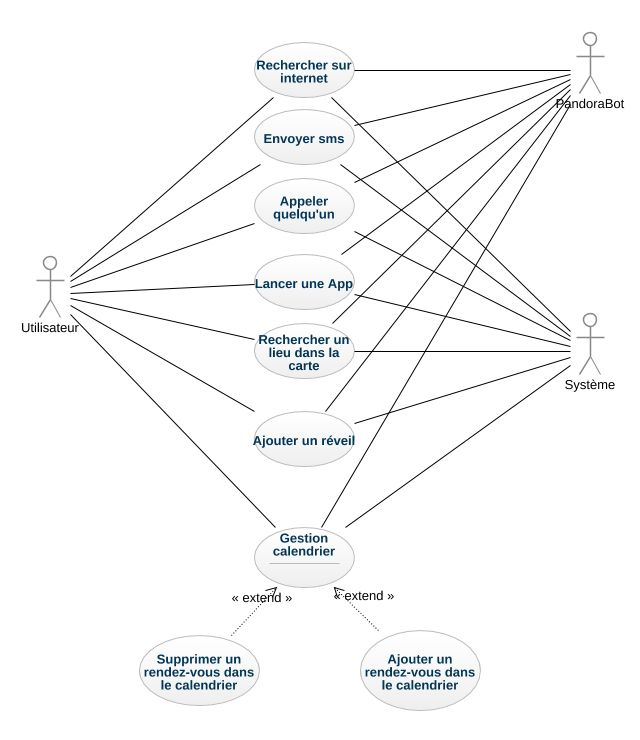
\includegraphics[scale=0.5]{./diagrammes/UsecaseDiagram.jpeg}
\caption{Diagramme de cas d'utilisation.\label{fig2}}
\end{figure}

\subsection{Diagramme de Sequence}
\begin{figure}[ht]
\centering
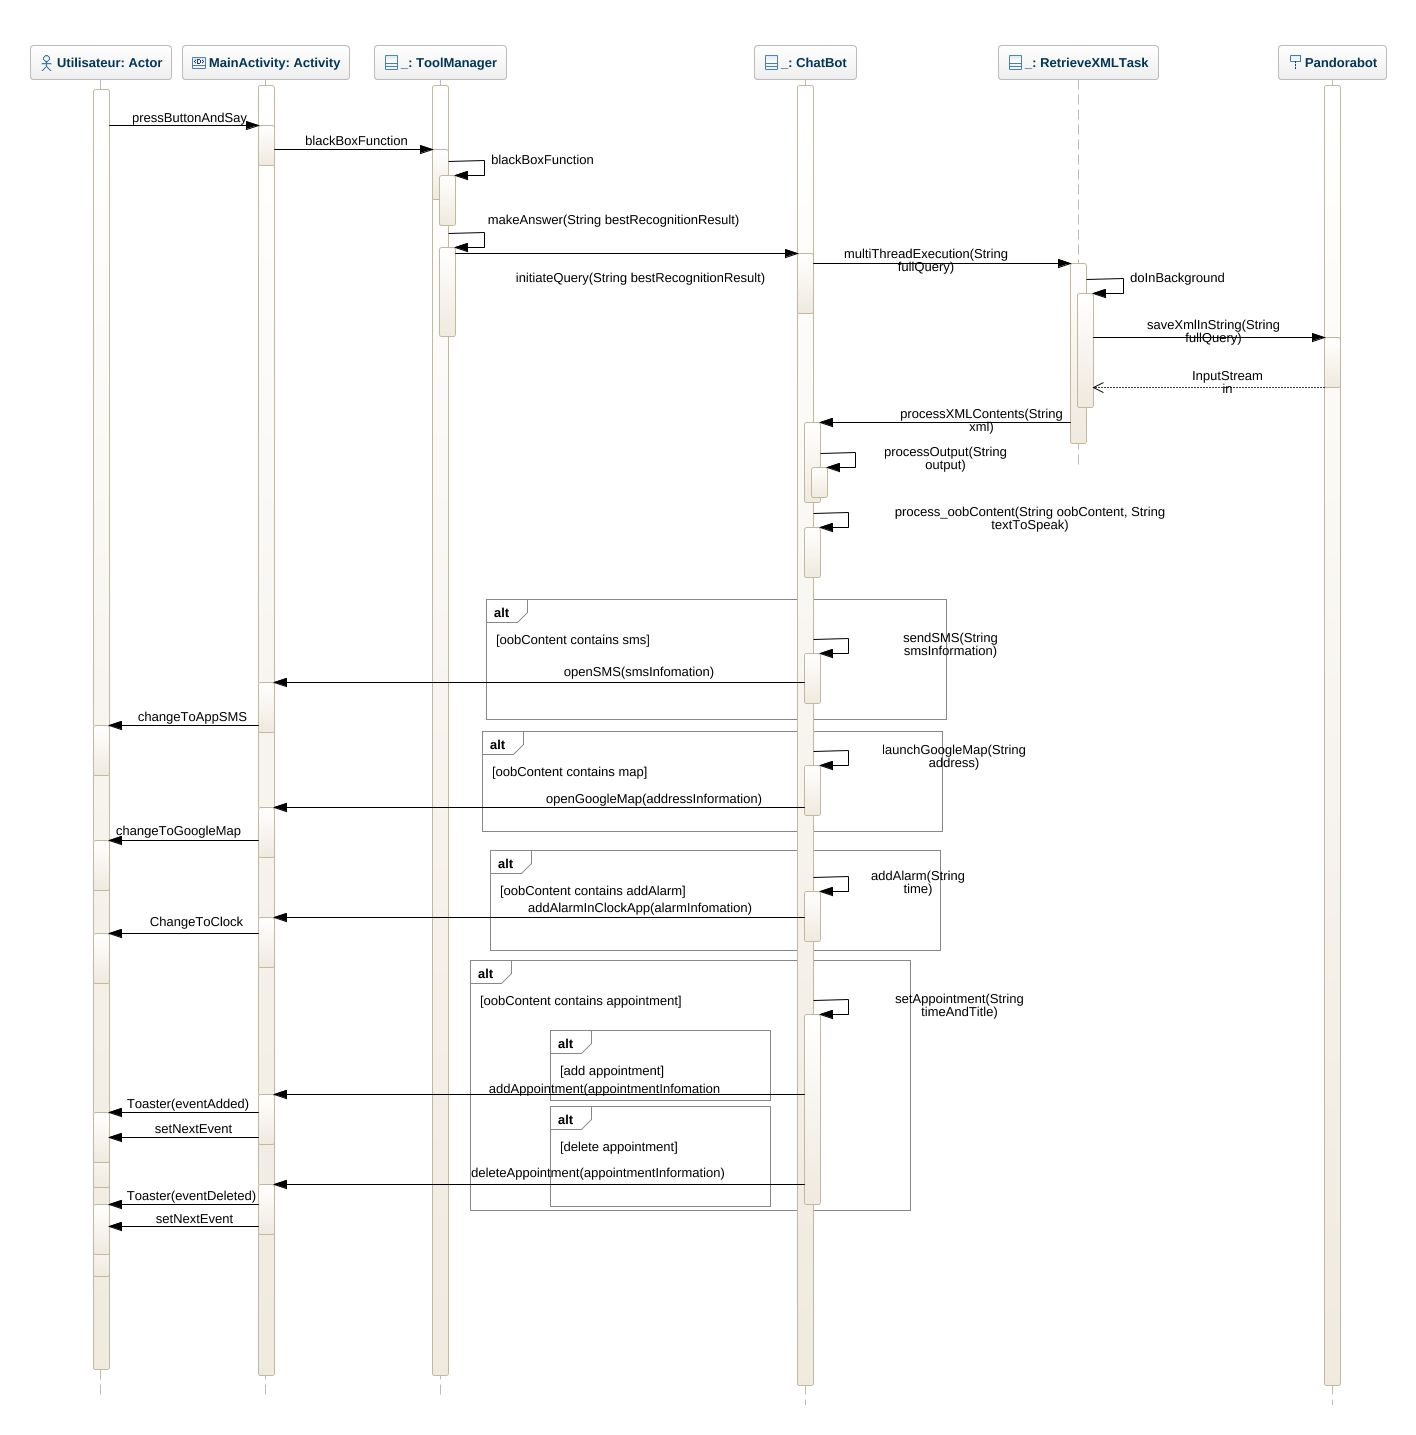
\includegraphics[scale=0.4]{./diagrammes/SequenceDiagram.jpeg}
\caption{Diagramme de Sequence.\label{fig3}}
\end{figure}
\indent La FIGURE \ref{fig3} représente un diagramme de séquence pour les fonctionnalités que nous avons proposé de réaliser. Les parties <<boite noire>> sont les parties du code qui ont été complétées dans les dernières versions. Ce que nous avons construit est la partie au-dessous de \textbf{\emph{process$_-$oobContent(String oobContent, String textToSpeak)}}.
\newpage

\subsection{Signatures Partie Chatbot}
procédure setAppointement (E/S Gcal : GestionCalendar, E oobContent : String, operationType : String)\\
\indent fonction setBeginTimeAndGetTitle (E oobContent : String, beginTime : Calendar, operationType : String) : String\\
\indent procédure googleQuery (E/S googleSearchText : String)\\
\indent procédure launchApp (E app : String)\\
\indent procédure launchUrl (E/S url : String)\\
\indent procédure launchGoogleMap (E/S address : String)\\
\indent procédure sendSMS (E oobContent : String)\\
\indent procédure makePhoneCall (E oobContent : String)\\
\indent procédure addAnAlarm(E oobContent : String)\\
\indent procédure deleteAnAlarm (E oobContent : String)\\

\subsection{Signatures Partie ToolManager}
procédure setNextEvent()\\
\indent fonction getNextEvent() : String\\
\newpage

